\documentclass[conference]{IEEEtran}
\IEEEoverridecommandlockouts
\usepackage{cite}
\usepackage{amsmath,amssymb,amsfonts}
\usepackage{algorithmic}
\usepackage{graphicx}
\usepackage{textcomp}
\usepackage{xcolor}
\usepackage{hyperref}
\usepackage{fontawesome5}
\usepackage{float}
\usepackage[section]{placeins}

\def\BibTeX{{\rm B\kern-.05em{\sc i\kern-.025em b}\kern-.08em
T\kern-.1667em\lower.7ex\hbox{E}\kern-.125emX}}
\begin{document}

    \title{Developing a Parallelized Genetic Algorithm Library using OpenMP, MPI, and CUDA\\}

    \author{
        \IEEEauthorblockN{Solomiia Gadiichuk}
        \IEEEauthorblockA{\textit{Faculty of Applied Sciences} \\
        Ukrainian Catholic University\\
        Lviv, Ukraine \\
        hadiichuk.pn@ucu.edu.ua}
        \and
        \IEEEauthorblockN{Bohdan Zasymovych}
        \IEEEauthorblockA{\textit{Faculty of Applied Sciences} \\
        Ukrainian Catholic University\\
        Lviv, Ukraine\\
        zasymovych.pn@ucu.edu.ua}
        \and
        \IEEEauthorblockN{Marta Kosiv}
        \IEEEauthorblockA{\textit{Faculty of Applied Sciences} \\
        Ukrainian Catholic University\\
        Lviv, Ukraine\\
        kosiv.pn@ucu.edu.ua}
        \and
        \IEEEauthorblockN{Mykola Balyk}
        \IEEEauthorblockA{\textit{Faculty of Applied Sciences} \\
        Ukrainian Catholic University\\
        Lviv, Ukraine\\
        balyk.pn@ucu.edu.ua}
    }

    \maketitle

    \begin{abstract}
        While Genetic Algorithms (GAs) are powerful optimization tools, their high computational cost limits scalability. This paper details the development of a genetic algorithm library that includes shared-memory, distributed-memory, and accelerator-based parallelization strategies to solve this problem. We describe an implemented multi-threaded Generational GA, a CUDA-accelerated GA, an MPI-based Island Model, a oneTBB-parallelized Cellular GA, and an OpenMP-optimized Differential Evolution algorithm. The performance of this library is evaluated using 3D mathematical surfaces and high-dimensional polygon image approximation tasks.
    \end{abstract}

    \begin{IEEEkeywords}
        Genetic Algorithms, Parallel Computing, Software Library, OpenMP, MPI, AVX, CUDA, Optimization
    \end{IEEEkeywords}

    \section{Introduction}
    Evolutionary algorithms are useful for solving complex optimization problems where traditional methods fail or take too much time. However, evaluating fitness functions for large populations over many generations requires a lot of computing power. 

    To solve this, different parallelization methods can be used, depending on the hardware and the specific algorithm. This project aims to develop a fast C++ library that includes four different algorithms: a classic Generational GA, an Island Model GA, a Cellular GA, and Differential Evolution (DE). Using tools like OpenMP, OpenMPI, oneTBB, and CUDA, we adapted these algorithms to the best hardware options (shared memory, distributed memory, and GPUs). 

    This paper presents the final implementation of the library, covering a diverse set of parallelized evolutionary models. It details the multi-threaded Generational GA, the CUDA-accelerated backend, the MPI-based Island Model, the oneTBB-parallelized Cellular GA, and the OpenMP-optimized Differential Evolution. The source code is publicly available at \faGithub\ \href{https://github.com/Martik-k/GALib-Parallel}{our GitHub}, and the full library documentation can be found \faBook\ \href{https://martik-k.github.io/GALib-Parallel/}{here}.

    \section{Background and Preliminaries}

    Genetic algorithms (GAs) are search and optimization methods inspired by natural evolution. Unlike standard algorithms that often get trapped in a local optimum, GAs use probability to explore large search spaces by evolving a population of possible solutions over several generations. This allows them to effectively escape local traps and find the true global maximum (or minimum) of a problem.

    \subsection{Representation and Fitness}
    Every possible solution in a GA is represented as a sequence of parameters called a \textit{chromosome} (or \textit{genotype}). Each individual parameter within this sequence is referred to as a \textit{gene}. In our real-coded implementation, genes are represented as floating-point values. How this solution actually looks or works in the problem is the \textit{phenotype}. Each solution is evaluated using a \textit{fitness function}, $F(x)$, which gives a score based on how well it solves the problem. The main goal of the algorithm is to find a chromosome with the highest (or lowest) fitness score.

    \subsection{Evolutionary Operators}
    Moving from one generation to the next uses three main steps \cite{b1}:
    \begin{itemize}
        \item \textbf{Selection:} The selection process determines which individuals from the current population will be chosen as parents to create the next generation.
        \item \textbf{Crossover:} Selected pairs exchange parts of their chromosome to create offspring. This combines the best traits from different parents.
        \item \textbf{Mutation:} It introduces random changes to the genetic material of the offspring solutions, helping to maintain diversity in the population and explore new regions of the search space.
    \end{itemize}

    \subsection{Schema Theory and Premature Convergence}
        The mathematical foundation of Genetic Algorithms is based on \textit{schemas}---templates that describe a subset of chromosomes sharing specific genes \cite{b2, b3}.

        \begin{itemize}
            \item \textbf{Binary Case:} A schema uses ones, zeros, and a "don't care" symbol ($*$). For example, the schema \texttt{1*0} matches both \texttt{110} and \texttt{100}.
            \item \textbf{Real-Valued Case:} In our implementation, because single-point crossover preserves exact numbers without blending them, floating-point values act as discrete symbols. Therefore, an exact numerical schema like $[1.52, *, 3.14]$ is valid and functions as a stable building block.
        \end{itemize}

        The growth of these schemas is described by Holland's Schema Theorem:
        \begin{equation}
            m(H, t+1) \ge m(H, t) \cdot \frac{f(H)}{\bar{f}} \left[ 1 - p_c \frac{\delta(H)}{L-1} - o(H)p_m \right]
        \end{equation}

        The components of this formula are defined as follows:
        \begin{itemize}
            \item $m(H, t)$: The number of instances of schema $H$ at generation $t$.
            \item $f(H)$: The average fitness of the schema $H$.
            \item $\bar{f}$: The average fitness of the entire population.
            \item $p_c$: The probability of crossover.
            \item $p_m$: The probability of mutation.
            \item $\delta(H)$: The defining length (the distance between the first and last fixed gene).
            \item $o(H)$: The order (the total number of fixed genes).
            \item $L$: The total length of the chromosome.
        \end{itemize}

    This theorem mathematically proves that schemas which are short (fixed genes are close together), low-order (few fixed genes), and possess above-average fitness will grow exponentially in the population over successive generations. By combining these highly fit building blocks, the algorithm efficiently avoids local traps and converges toward the global maximum.

    \section{Software Architecture and Design}
    The library is designed as a high-performance, header-only C++20 framework. Its architecture prioritizes performance through modern C++ features while maintaining high extensibility for research and industrial applications.

    \subsection{Template-Driven Extensibility}
    GALib-Parallel utilizes C++20 templates to allow for type-safe and performant gene representations. While primarily focused on double-precision floating-point values for continuous optimization, the template-based design ensures that the core evolutionary logic remains decoupled from specific data types. This approach eliminates the overhead of virtual function calls in hot paths (such as gene-level operations) and allows for aggressive compiler optimizations like inlining and SIMD vectorization.

    \subsection{Interface-Based Design}
    The framework is built upon a set of abstract interfaces that define the contract for evolutionary components. This modularity allows users to extend the library with custom logic by implementing specialized classes for:
    \begin{itemize}
        \item \textbf{Algorithm:} The core orchestrator for different evolutionary models (Standard, Island, Cellular, DE).
        \item \textbf{Selection, Crossover, and Mutation:} Generic operators for offspring generation.
        \item \textbf{Topology, DemeSelector, and DemeReplacer:} Specialized components for the Island Model's migration dynamics.
        \item \textbf{FitnessFunction:} The objective function to be minimized, supporting both standard inheritance and functional (lambda-based) wrappers.
    \end{itemize}

    \section{Evolutionary Operators and Components}
    This section describes the specific evolutionary strategies and components implemented within the library.

    \subsection{Genetic Operators}
    The library provides a variety of genetic operators to handle diverse optimization landscapes:
    \begin{itemize}
        \item \textbf{Selection:} Supports Tournament Selection, which maintains high selection pressure without requiring a full population sort, facilitating parallel execution.
        \item \textbf{Crossover:} Includes Single-Point, Uniform, and Arithmetic Crossover. Arithmetic crossover is particularly effective for real-coded GAs as it produces offspring within the convex hull of the parents.
        \item \textbf{Mutation:} Implements Gaussian Mutation for fine-grained local search, Uniform Mutation for global exploration, and Boundary Mutation to handle search space constraints.
    \end{itemize}

    \subsection{Island Model Migration Dynamics}
    The Island Model utilizes specialized components to manage the exchange of genetic material between subpopulations, following the theoretical foundations of the Generalized Island Model \cite{b4}:
    \begin{itemize}
        \item \textbf{Migration Topologies:} Defines the connectivity of the archipelago. Implemented topologies include One-Way Ring, Bidirectional Ring, and Fully Connected graphs, each offering different trade-offs between information spread and diversity preservation \cite{b6}.
        \item \textbf{Migration Selectors (DemeSelector):} Responsible for choosing individuals for migration. The Elitism Selector is commonly used to share the best local traits across the cluster.
        \item \textbf{Migration Replacers (DemeReplacer):} Determines how migrants are integrated. The Worst Replacer strategy ensures that incoming high-fitness individuals replace the least fit local members, driving the subpopulation toward the global optimum while maintaining diversity \cite{b5}.
    \end{itemize}

    \subsection{Benchmark Functions}
    The library includes several built-in fitness functions for validation and benchmarking \cite{b6}. These include unimodal functions like the Sphere function, multi-modal problems such as Rastrigin and Himmelblau, and specialized benchmarks like De Jong's Foxholes. Additionally, a computationally intensive HeavyTrig function is provided specifically to evaluate the library's parallel scaling performance under significant computational loads.

    \section{Parallel Algorithmic Models}
    
    \subsection{Generational Genetic Algorithm}
    The Generational Genetic Algorithm follows a classic evolutionary cycle, refined for continuous optimization as a Real-Coded Genetic Algorithm (RCGA).

    \subsubsection{Standard Parallel Implementation}
    The implementation utilizes shared-memory parallelism via OpenMP to accelerate the evolutionary loop. The algorithm consists of the following data-parallel stages:
    \begin{itemize}
        \item \textbf{Initialization:} The initial population is generated randomly across the search space. Local random number generators are used per thread to ensure thread-safety and avoid bottlenecking on global state.
        \item \textbf{Evaluation:} The fitness of each individual is computed independently. This computationally intensive phase is parallelized using \texttt{\#pragma omp parallel for}, distributing the workload across multiple CPU cores.
        \item \textbf{Selection:} Parents are identified based on their fitness scores. This stage is executed in parallel, allowing for rapid parent selection across the population.
        \item \textbf{Crossover and Mutation:} New offspring are created and mutated in parallel, maximizing throughput by utilizing all available hardware threads.
    \end{itemize}

    \subsubsection{CUDA-Accelerated Backend}
    We implemented a CUDA backend for the generational GA to accelerate its most expensive data-parallel stages: fitness evaluation, crossover, mutation, and elite selection. The implementation uses dedicated CUDA kernels, stateless on-device random generation, FP32 internal computation with CUDA fast math, and a resident device population to minimize host-device transfers.

    \subsection{Differential Evolution}
    Differential Evolution (DE) is implemented for efficient optimization of continuous variables. Unlike traditional mutation operators, DE generates new candidate solutions by taking the difference between randomly selected individuals in the population. The mutation strategy used is DE/rand/1.

    Selection is performed by comparing the fitness of $u_i$ and $x_i$, keeping the better one. This adaptive search mechanism allows DE to converge faster than traditional GAs on many optimization problems. The implementation uses OpenMP for parallel evaluation of the population and SIMD vectorization for the mutation and crossover steps.

    \subsection{Island Model Genetic Algorithm}
    The Island Model, or coarse-grained parallel GA, partitions the total population into several semi-isolated subpopulations known as islands. Each island evolves independently according to its own local parameters, such as mutation and crossover rates. This independence allows different islands to explore diverse regions of the search space simultaneously, effectively acting as a mechanism to preserve genetic diversity and prevent premature convergence. 

    \subsubsection{Parallelization and MPI Communication}
    The implementation utilizes a multi-tiered parallelization strategy to maximize hardware utilization across compute clusters. At the local level, shared-memory parallelism is employed to accelerate fitness evaluations and the creation of offspring within each island. At the distributed level, the Message Passing Interface (MPI) handles the coordination and data transfer between separate processes. 

    The communication layer utilizes an asynchronous design, employing non-blocking MPI primitives and thread-safe circular buffers. This allows islands to continue their evolutionary cycles without being stalled by network latency or waiting for synchronization with peers. Migrants are serialized into a portable binary format for efficient transmission and are processed by the destination island at the start of its next generation. Additionally, occasional global synchronization points allow for the identification and sharing of the absolute best solution found across the entire archipelago, ensuring that all nodes eventually converge on the global optimum.

    \subsection{Cellular Genetic Algorithm}
    In the implemented Cellular Genetic Algorithm, the population is treated as a two-dimensional toroidal grid whose shape is inferred automatically from the total population size by selecting a factorization close to a square. Each cell stores one individual, and reproduction is restricted to local interaction: one parent is the current individual, while the second parent is selected from the Von Neumann neighborhood consisting of the four adjacent cells (up, down, left, and right) with wrap-around boundary conditions.

    Parent selection is performed by choosing the fittest neighboring individual. The selected pair then undergoes crossover with probability $p_c$ and mutation with probability $p_m$, producing two offspring that are evaluated immediately. If local elitism is enabled, the algorithm preserves the best individual among the current parent and the two offspring; otherwise, only the better offspring survives. The resulting individuals are written into a temporary population, and the old population is replaced synchronously after all cells have been processed. This local interaction pattern helps preserve spatial diversity and slows premature convergence compared to fully panmictic population models. Both the initial population evaluation and the cell-wise update phase are parallelized with oneTBB through \texttt{tbb::parallel\_for}. This parallelization is safe because each task reads individuals only from the previous generation state and writes its result into an independent slot of the temporary population, thereby avoiding write conflicts during the generation update.

    \section{Benchmarks}

    \subsection{Comparison of CUDA and Parallel Standard GA}
    We compared the CUDA-accelerated backend against the multi-threaded OpenMP implementation on an NVIDIA GeForce RTX 4050 GPU using the HeavyTrig benchmark. As shown in Figure~\ref{fig:cuda_ga_speedup}, the GPU provides a substantial advantage for compute-intensive workloads, achieving speedups between 3.70$\times$ and 12.04$\times$ depending on population size and complexity.

    \begin{figure}[H]
        \centering
        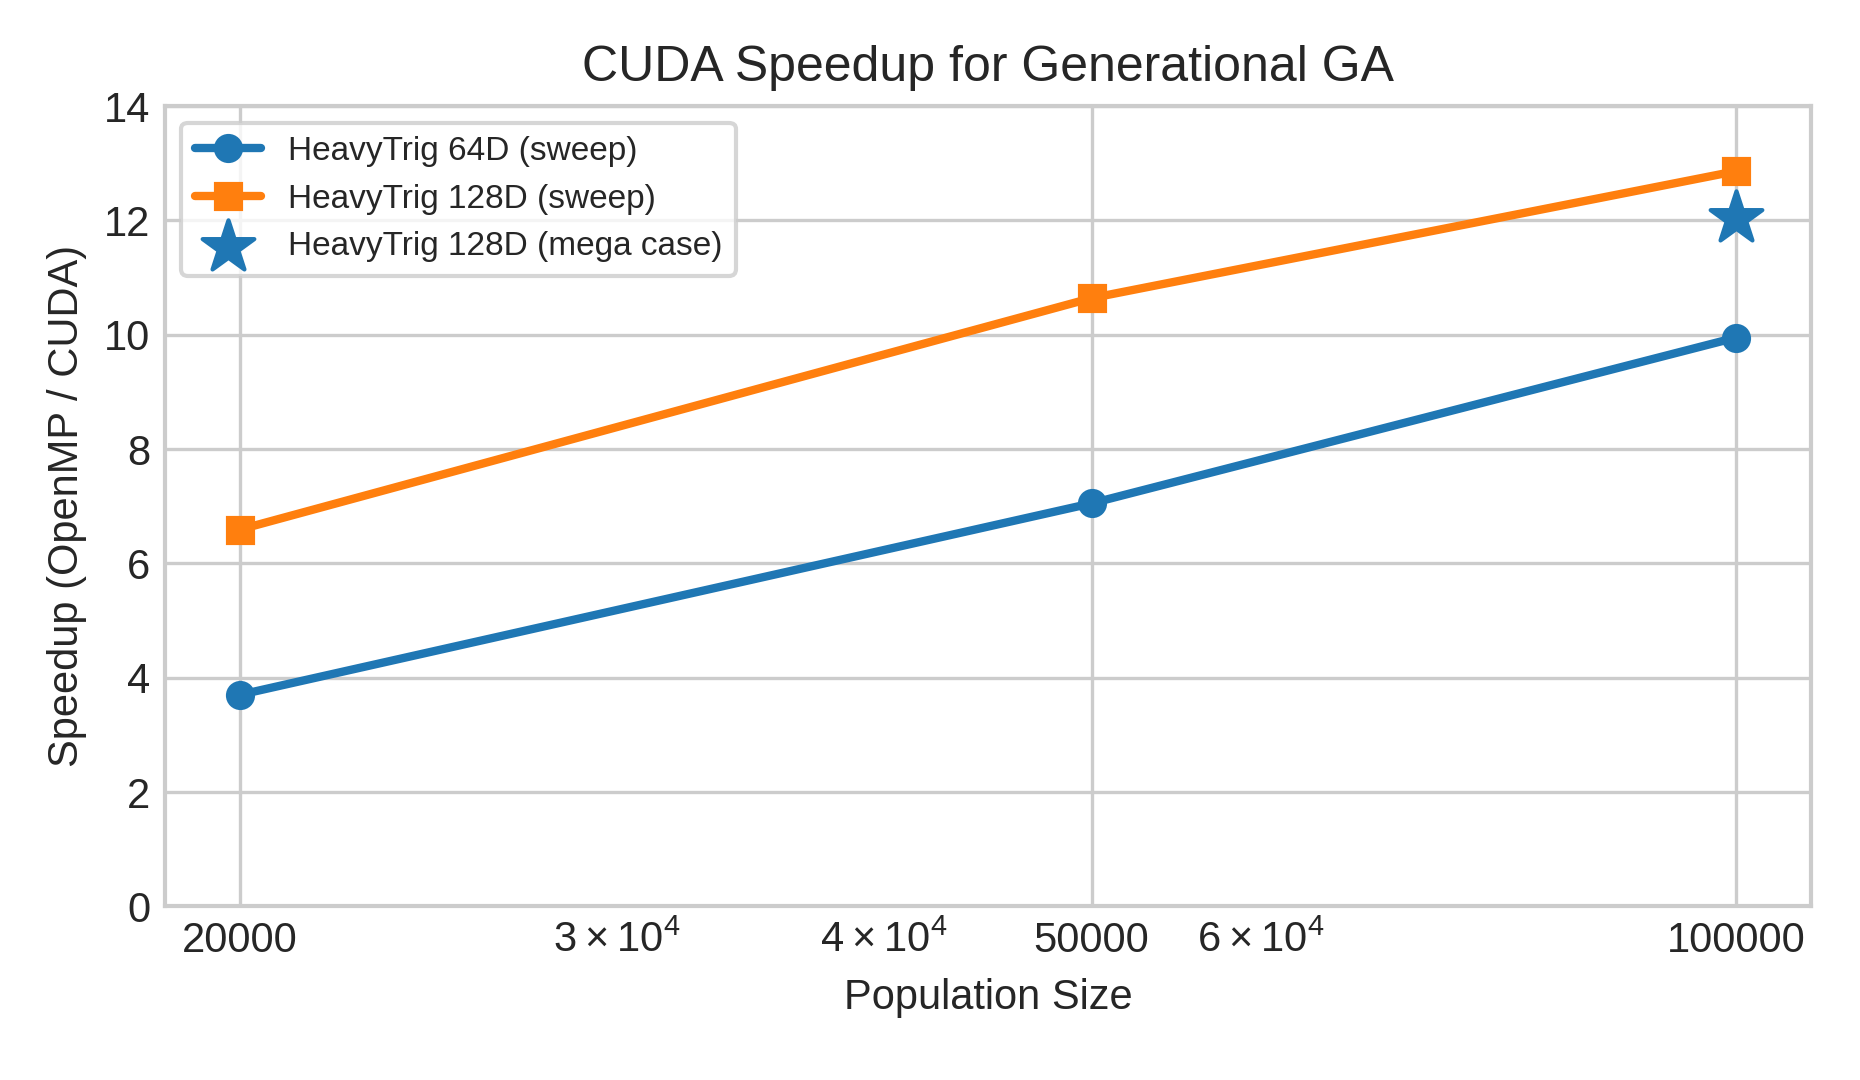
\includegraphics[width=\columnwidth]{media/cuda_ga_speedup.png}
        \caption{CUDA speedup for Generational GA on HeavyTrig benchmark.}
        \label{fig:cuda_ga_speedup}
    \end{figure}

    \subsection{Hybrid Island GA Cluster Scaling}
    The scalability of the Hybrid Island Model was evaluated on a heterogeneous cluster of three nodes (18 cores total). 

    \subsubsection{Hardware Specifications}
    The benchmark was conducted on three physical machines with the following hardware configurations:
    \begin{itemize}
        \item \textbf{Worker 1:} 8 physical cores @ [Freq] GHz, [Size] GB [Type] RAM @ [Speed] MHz.
        \item \textbf{Worker 2:} 6 physical cores @ 3.3 GHz, 16 GB DDR5 RAM @ 4800 MHz.
        \item \textbf{Worker 3:} 4 physical cores @ [Freq] GHz, [Size] GB [Type] RAM @ [Speed] MHz.
    \end{itemize}

    \subsubsection{Methodology and Load Balancing}
    To demonstrate strong scaling with a fixed workload of 9 islands, we utilized a proportional load balancing strategy. Islands were assigned based on core counts (4:3:2) to ensure each island had equal compute resources (2 cores) and reached synchronization points simultaneously, maximizing cluster efficiency.

    \subsubsection{Experimental Results}
    Scaling performance was measured across three hardware tiers, with results summarized in Figure~\ref{fig:cluster_bench}. The hybrid architecture demonstrated effective scaling; transition to a two-machine configuration (14 cores) yielded a 2.02$\times$ speedup over the single-node baseline. The full 18-core cluster further improved performance, reaching a 2.32$\times$ total speedup.

    \begin{figure}[H]
        \centering
        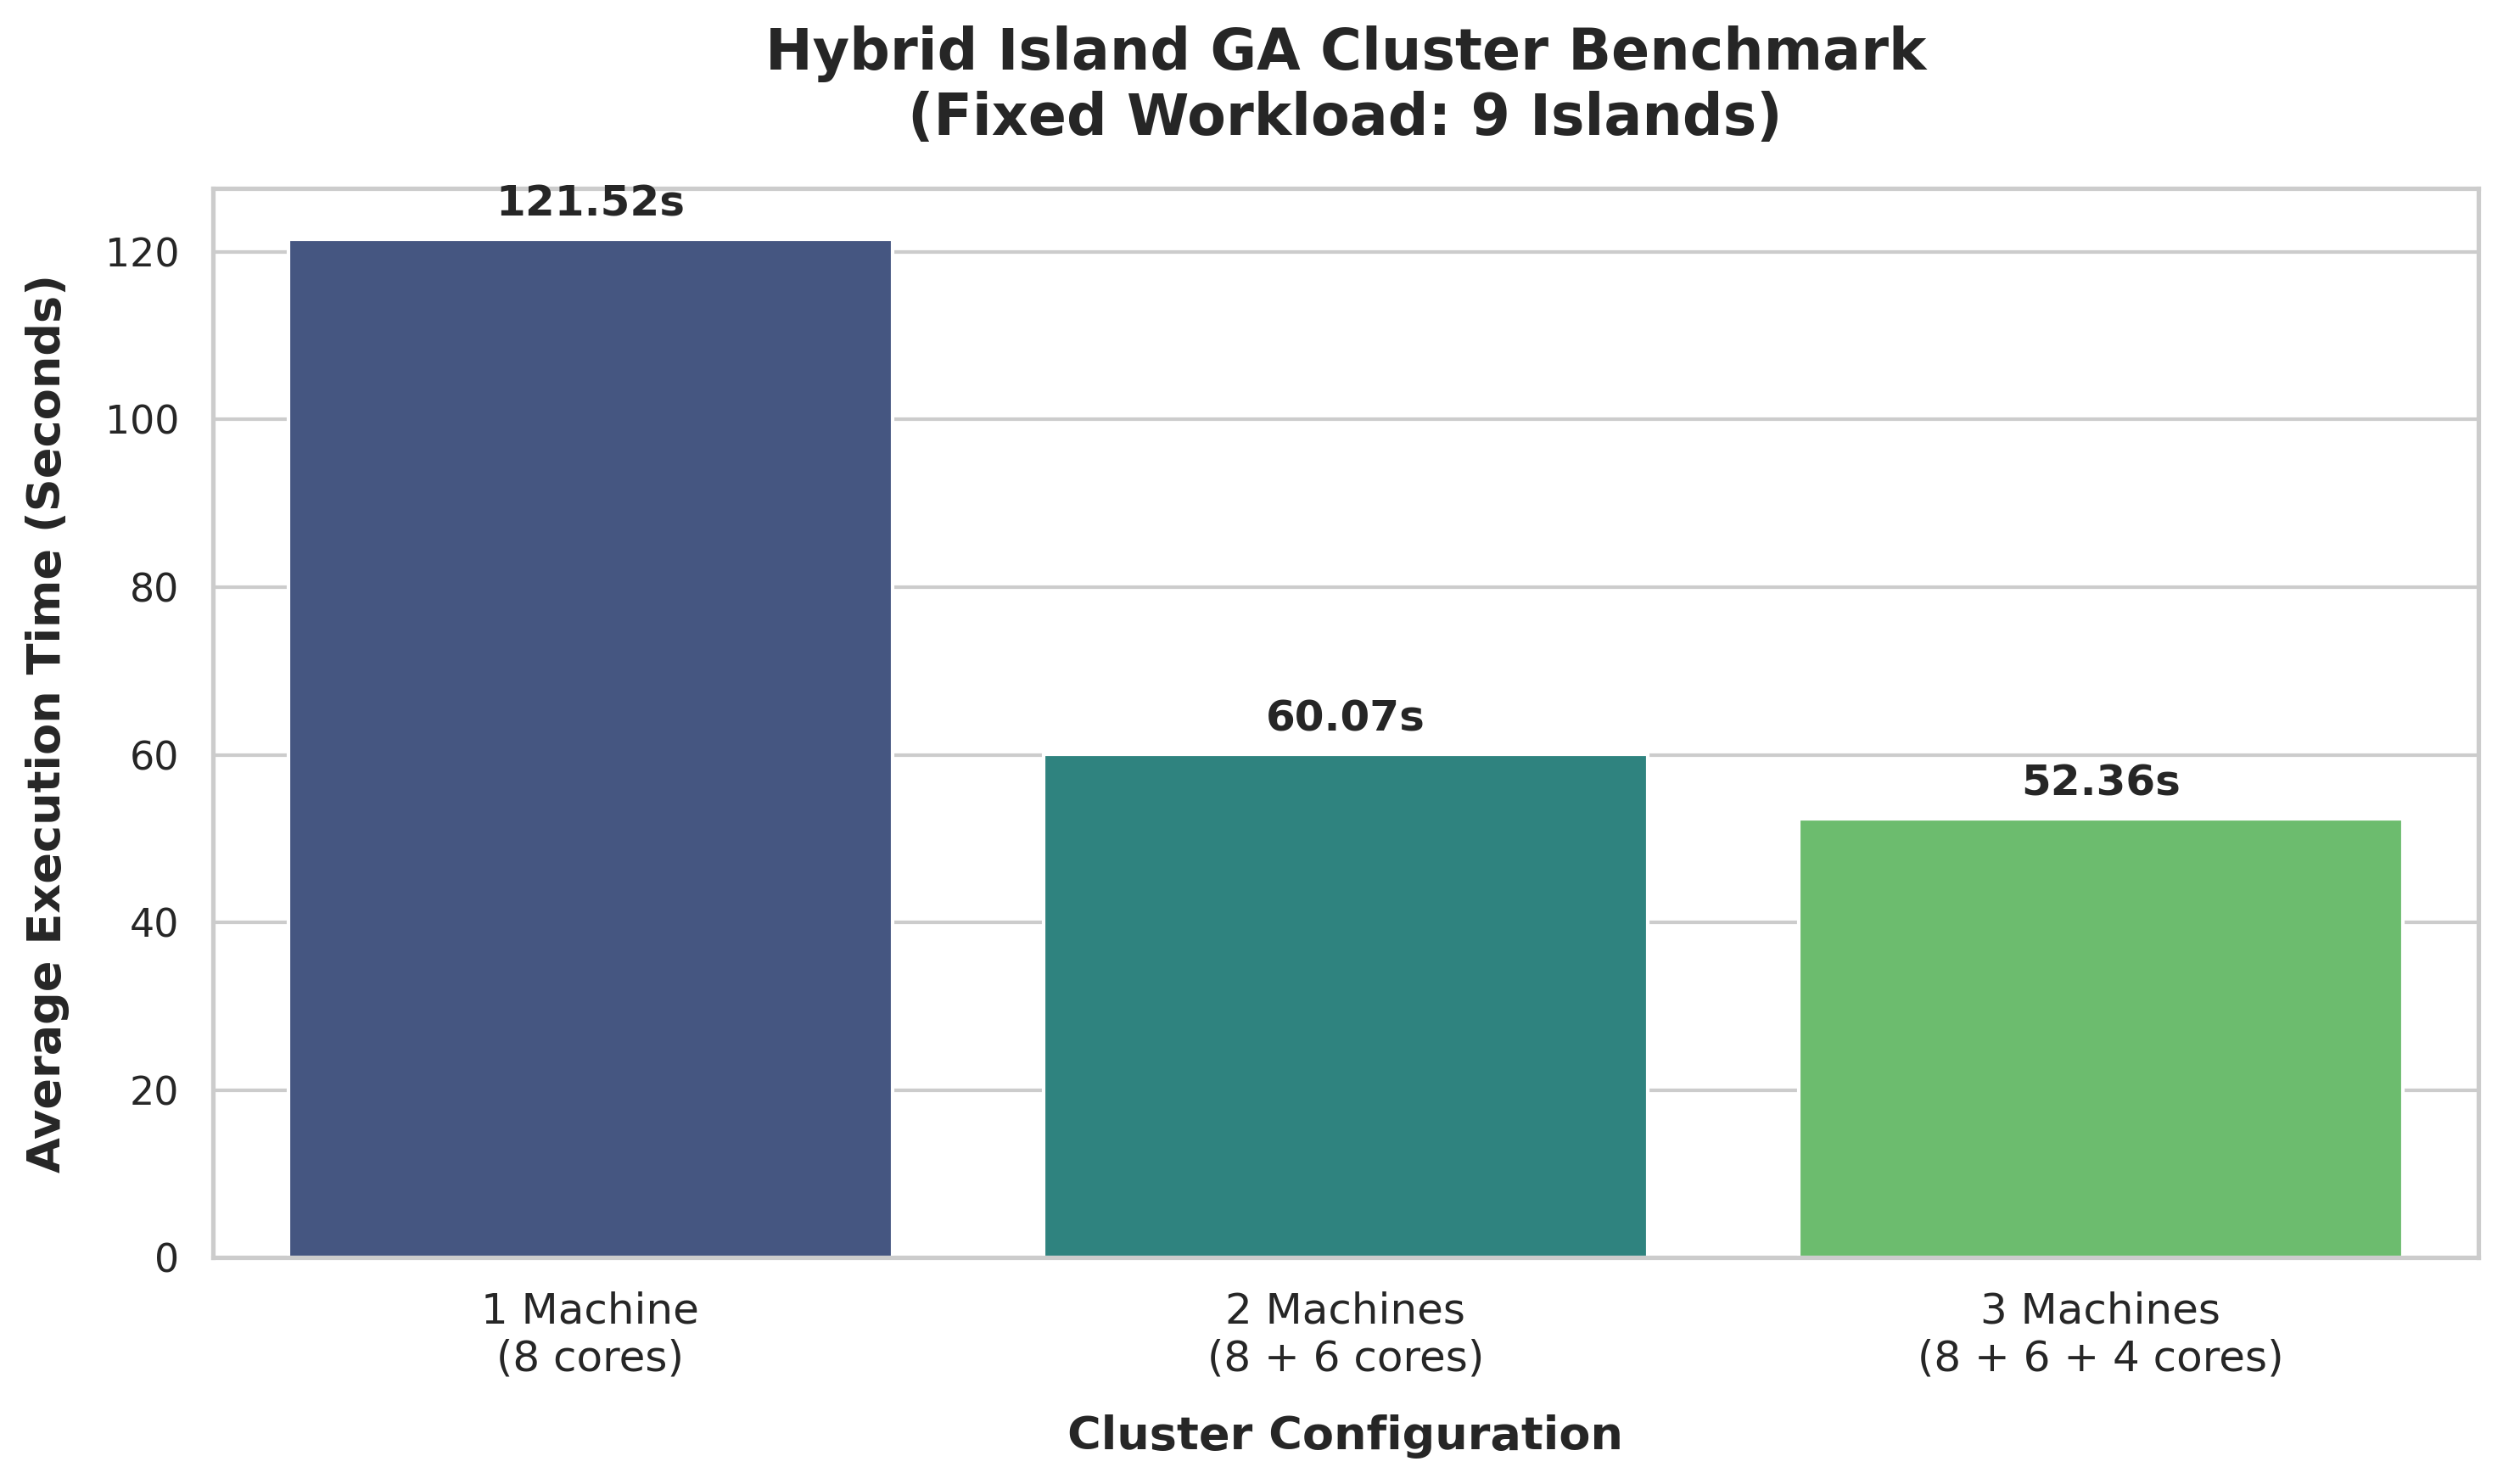
\includegraphics[width=\columnwidth]{media/cluster_benchmark_plot.png}
        \caption{Strong scaling results for the Hybrid Island GA across the heterogeneous cluster.}
        \label{fig:cluster_bench}
    \end{figure}

    \section{Library Usage}
    
    \subsection{Installation and Compilation}
    GALib-Parallel is distributed as a CMake-based C++20 library whose standard workflow follows the configure--build--install model. During configuration, CMake automatically detects optional dependencies such as MPI and the CUDA Toolkit and enables the corresponding exported targets only when the required environment is available; consequently, the base package is always provided through \texttt{GALib::ga\_lib}, while \texttt{GALib::ga\_cuda} and \texttt{GALib::ga\_island} are exposed only in CUDA- and MPI-enabled builds, respectively. The installation exports public headers, package configuration files, sample configurations, and example sources, allowing downstream users to integrate the library through \texttt{find\_package(GALib)}. The practical build, installation, and linking steps are described in the \href{https://martik-k.github.io/GALib-Parallel/}{library documentation} and main project page.

    \subsection{User API and Programming Model}
    The library provides a high-level, data-driven API designed to minimize boilerplate. The programming model follows three primary stages: problem definition, engine instantiation, and evolution.

    \subsubsection{Problem Definition}
    Users define optimization problems by implementing the \texttt{FitnessFunction} interface or, more conveniently, by using the \texttt{FunctionalFitness} wrapper. The latter allows for inline problem definition using C++ lambdas, as shown in the example below.

    \subsubsection{Engine Instantiation}
    The library supports two modes of instantiation:
    \begin{itemize}
        \item \textbf{Configuration-Driven (Recommended):} The \texttt{AlgorithmBuilder} factory parses a YAML file and automatically assembles the requested algorithm (Standard, Island, etc.) with its corresponding operators and parameters.
        \item \textbf{Manual Construction:} For specialized use cases, users can manually instantiate algorithms (e.g., \texttt{StandardGA}) by passing operator unique pointers and parameter structures directly to the constructor.
    \end{itemize}

    \subsubsection{Configuration Parameters}
    The YAML configuration system centralizes algorithm behavior. Key parameters include:
    \begin{itemize}
        \item \textbf{threads:} Sets the OpenMP thread count (0 for system maximum).
        \item \textbf{max\_generations:} Evolution limit.
        \item \textbf{mutation\_rate} and \textbf{crossover\_rate:} Operator probabilities.
        \item \textbf{selection/mutation/crossover:} Type-based operator selection.
    \end{itemize}

    \subsubsection{Minimal Usage Example}
    The following snippet demonstrates the complete workflow for a 2D minimization task:

    \begin{figure}[H]
        \begin{minipage}{\columnwidth}
\begin{verbatim}
// 1. Define problem via lambda
FunctionalFitness<double> fitness(2, -5.0, 5.0, 
    [](const std::vector<double>& p) {
        return p[0]*p[0] + p[1]*p[1];
    });

// 2. Build algorithm from YAML config
auto ga = utils::AlgorithmBuilder<double>::build(
    "config.yaml", fitness);

// 3. Evolve population
Population<double> pop(100, 2);
pop.initialize(fitness.getLowerBound(), 
               fitness.getUpperBound());
ga->run(pop);

// 4. Get results
std::cout
    << "Best Fitness: "
    << pop.getBestIndividual().getFitness();
\end{verbatim}
        \end{minipage}
        \caption{Minimal GALib-Parallel usage example.}
    \end{figure}

    \section{Conclusion}

    \section*{Acknowledgment}

    \begin{thebibliography}{00}
        \bibitem{b1} ``Real-Coded Genetic Algorithm,'' \textit{Algorithm Afternoon}, [Online]. Available: \url{https://algorithmafternoon.com/genetic/real_coded_genetic_algorithm/}. [Accessed: Mar. 5, 2026].
        
        \bibitem{b2} O. Farenyuk, ``Genetic Algorithms'' unpublished lecture notes.

        \bibitem{b3} ``Holland's schema theorem,'' \textit{Wikipedia}, [Online]. Available: \url{https://en.wikipedia.org/wiki/Holland%27s_schema_theorem}. [Accessed: Mar. 5, 2026].

        \bibitem{b4} D. Izzo, M. Ruci{\'n}ski, and F. Biscani, ``The Generalized Island Model,'' in \textit{Parallel Architectures and Bioinspired Algorithms}, Berlin, Heidelberg: Springer, 2012, pp. 151--169. doi: 10.1007/978-3-642-28789-3\_7.

        \bibitem{b5} A. A. Gozali and S. Fujimura, ``Localized Island Model Genetic Algorithm in Population Diversity Preservation,'' in \textit{Proceedings of the 2018 International Conference on Industrial Enterprise and System Engineering (IcoIESE 2018)}, 2019, pp. 122--128. doi: 10.2991/icoiese-18.2019.22.

        \bibitem{b6} D. Whitley, S. Rana, and R. B. Heckendorn, ``The Island Model Genetic Algorithm: On Separability, Population Size and Convergence,'' \textit{Journal of Computing and Information Technology}, vol. 7, no. 1, pp. 33--47, 1999. [Online].
    \end{thebibliography}
\end{document}
